% Created by tikzDevice version 0.12.6 on 2024-02-25 11:58:22
% !TEX encoding = UTF-8 Unicode
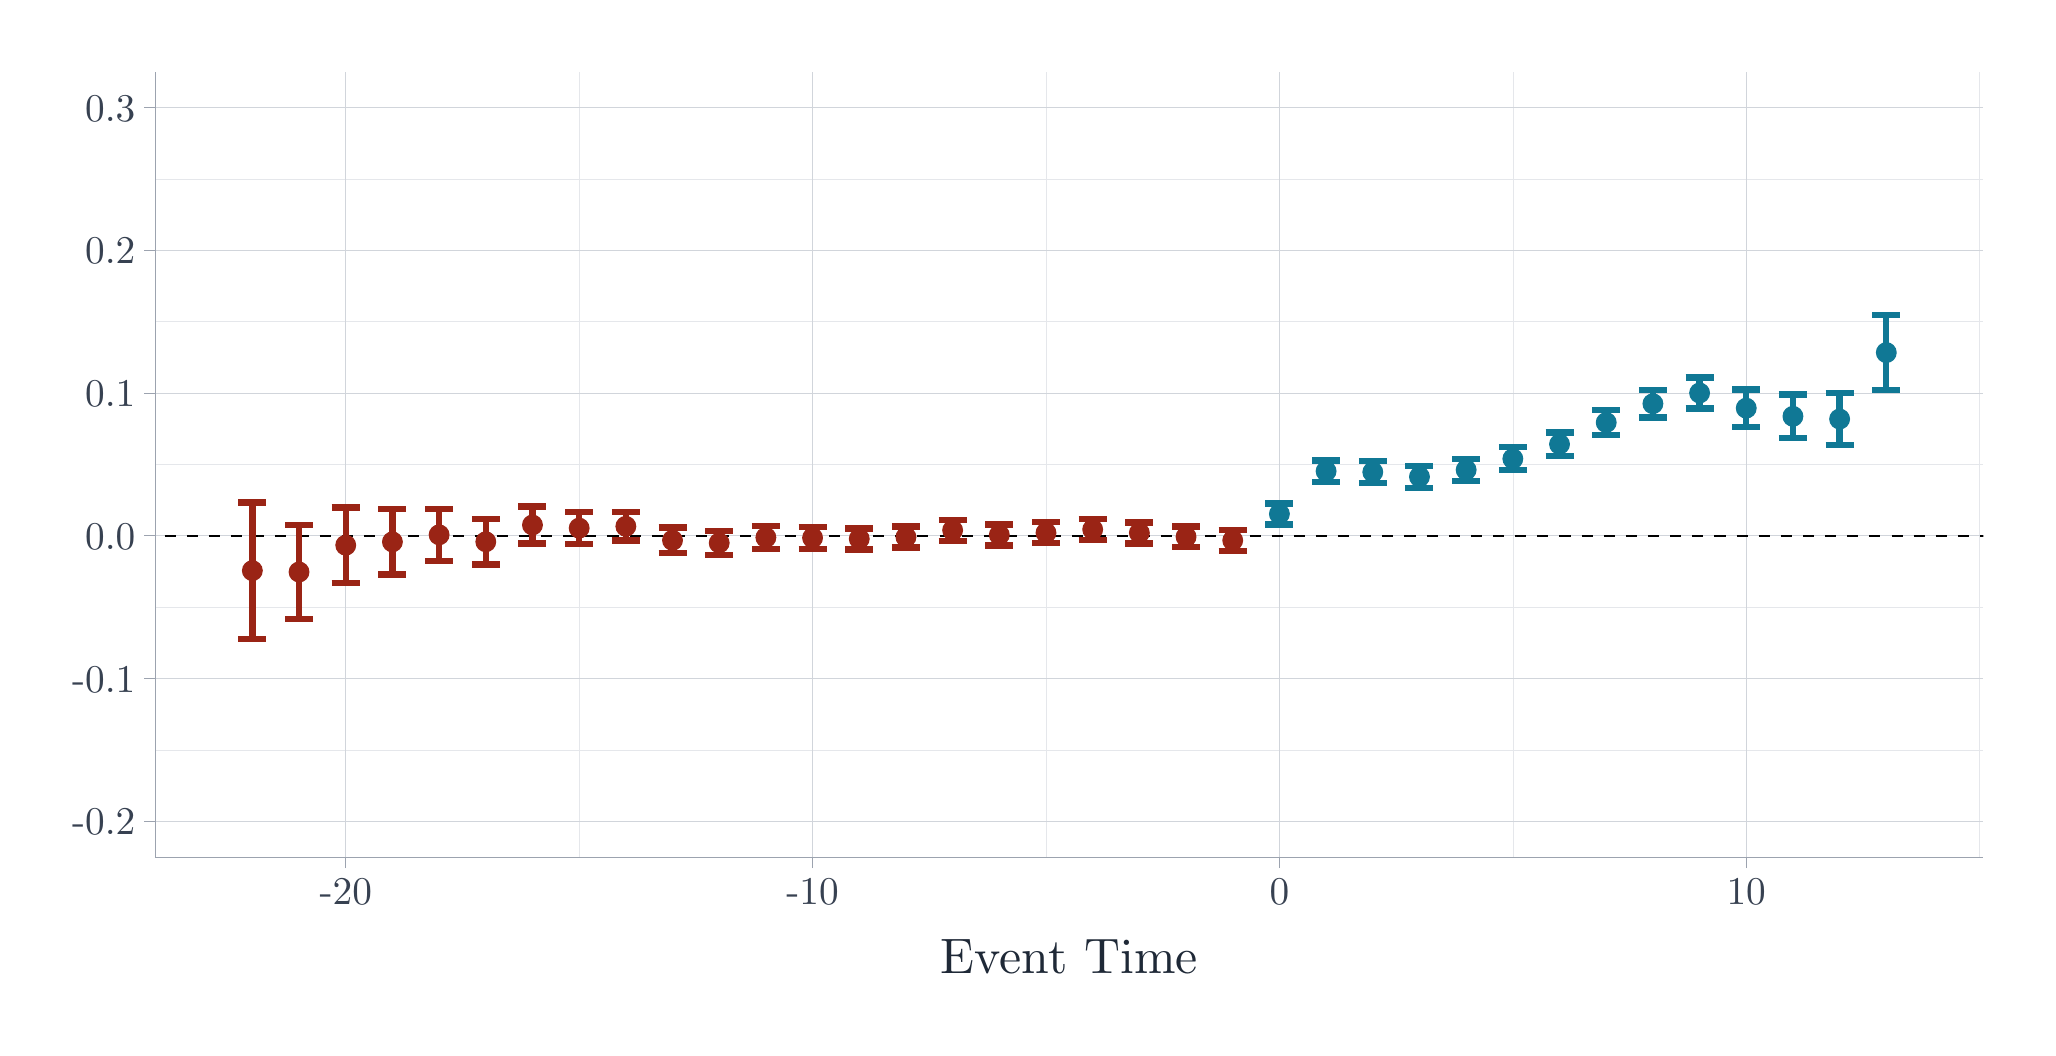
\begin{tikzpicture}[x=1pt,y=1pt]
\definecolor{fillColor}{RGB}{255,255,255}
\path[use as bounding box,fill=fillColor] (0,0) rectangle (722.70,361.35);
\begin{scope}
\path[clip] (  0.00,  0.00) rectangle (722.70,361.35);
\definecolor{drawColor}{RGB}{255,255,255}

\path[draw=drawColor,line width= 0.8pt,line join=round,line cap=round,fill=fillColor] (  0.00,  0.00) rectangle (722.70,361.35);
\end{scope}
\begin{scope}
\path[clip] ( 46.10, 61.65) rectangle (706.70,345.35);
\definecolor{drawColor}{RGB}{255,255,255}
\definecolor{fillColor}{RGB}{255,255,255}

\path[draw=drawColor,line width= 0.8pt,line join=round,line cap=round,fill=fillColor] ( 46.10, 61.65) rectangle (706.70,345.35);
\definecolor{drawColor}{RGB}{229,231,235}

\path[draw=drawColor,line width= 0.2pt,line join=round] ( 46.10,100.34) --
	(706.70,100.34);

\path[draw=drawColor,line width= 0.2pt,line join=round] ( 46.10,151.92) --
	(706.70,151.92);

\path[draw=drawColor,line width= 0.2pt,line join=round] ( 46.10,203.50) --
	(706.70,203.50);

\path[draw=drawColor,line width= 0.2pt,line join=round] ( 46.10,255.08) --
	(706.70,255.08);

\path[draw=drawColor,line width= 0.2pt,line join=round] ( 46.10,306.66) --
	(706.70,306.66);

\path[draw=drawColor,line width= 0.2pt,line join=round] (199.28, 61.65) --
	(199.28,345.35);

\path[draw=drawColor,line width= 0.2pt,line join=round] (367.97, 61.65) --
	(367.97,345.35);

\path[draw=drawColor,line width= 0.2pt,line join=round] (536.66, 61.65) --
	(536.66,345.35);

\path[draw=drawColor,line width= 0.2pt,line join=round] (705.35, 61.65) --
	(705.35,345.35);
\definecolor{drawColor}{RGB}{209,213,219}

\path[draw=drawColor,line width= 0.4pt,line join=round] ( 46.10, 74.55) --
	(706.70, 74.55);

\path[draw=drawColor,line width= 0.4pt,line join=round] ( 46.10,126.13) --
	(706.70,126.13);

\path[draw=drawColor,line width= 0.4pt,line join=round] ( 46.10,177.71) --
	(706.70,177.71);

\path[draw=drawColor,line width= 0.4pt,line join=round] ( 46.10,229.29) --
	(706.70,229.29);

\path[draw=drawColor,line width= 0.4pt,line join=round] ( 46.10,280.87) --
	(706.70,280.87);

\path[draw=drawColor,line width= 0.4pt,line join=round] ( 46.10,332.45) --
	(706.70,332.45);

\path[draw=drawColor,line width= 0.4pt,line join=round] (114.93, 61.65) --
	(114.93,345.35);

\path[draw=drawColor,line width= 0.4pt,line join=round] (283.62, 61.65) --
	(283.62,345.35);

\path[draw=drawColor,line width= 0.4pt,line join=round] (452.31, 61.65) --
	(452.31,345.35);

\path[draw=drawColor,line width= 0.4pt,line join=round] (621.00, 61.65) --
	(621.00,345.35);
\definecolor{drawColor}{RGB}{0,0,0}

\path[draw=drawColor,line width= 0.9pt,dash pattern=on 4pt off 4pt ,line join=round] (-614.49,177.71) -- (1367.30,177.71);
\definecolor{drawColor}{RGB}{154,36,21}
\definecolor{fillColor}{RGB}{154,36,21}

\path[draw=drawColor,line width= 0.4pt,line join=round,line cap=round,fill=fillColor] ( 81.19,165.14) circle (  3.57);

\path[draw=drawColor,line width= 0.4pt,line join=round,line cap=round,fill=fillColor] ( 98.06,164.66) circle (  3.57);

\path[draw=drawColor,line width= 0.4pt,line join=round,line cap=round,fill=fillColor] (114.93,174.34) circle (  3.57);

\path[draw=drawColor,line width= 0.4pt,line join=round,line cap=round,fill=fillColor] (131.80,175.54) circle (  3.57);

\path[draw=drawColor,line width= 0.4pt,line join=round,line cap=round,fill=fillColor] (148.67,178.09) circle (  3.57);

\path[draw=drawColor,line width= 0.4pt,line join=round,line cap=round,fill=fillColor] (165.54,175.58) circle (  3.57);

\path[draw=drawColor,line width= 0.4pt,line join=round,line cap=round,fill=fillColor] (182.41,181.64) circle (  3.57);

\path[draw=drawColor,line width= 0.4pt,line join=round,line cap=round,fill=fillColor] (199.28,180.51) circle (  3.57);

\path[draw=drawColor,line width= 0.4pt,line join=round,line cap=round,fill=fillColor] (216.15,181.16) circle (  3.57);

\path[draw=drawColor,line width= 0.4pt,line join=round,line cap=round,fill=fillColor] (233.01,176.11) circle (  3.57);

\path[draw=drawColor,line width= 0.4pt,line join=round,line cap=round,fill=fillColor] (249.88,175.15) circle (  3.57);

\path[draw=drawColor,line width= 0.4pt,line join=round,line cap=round,fill=fillColor] (266.75,177.12) circle (  3.57);

\path[draw=drawColor,line width= 0.4pt,line join=round,line cap=round,fill=fillColor] (283.62,177.00) circle (  3.57);

\path[draw=drawColor,line width= 0.4pt,line join=round,line cap=round,fill=fillColor] (300.49,176.64) circle (  3.57);

\path[draw=drawColor,line width= 0.4pt,line join=round,line cap=round,fill=fillColor] (317.36,177.27) circle (  3.57);

\path[draw=drawColor,line width= 0.4pt,line join=round,line cap=round,fill=fillColor] (334.23,179.76) circle (  3.57);

\path[draw=drawColor,line width= 0.4pt,line join=round,line cap=round,fill=fillColor] (351.10,178.06) circle (  3.57);

\path[draw=drawColor,line width= 0.4pt,line join=round,line cap=round,fill=fillColor] (367.97,178.83) circle (  3.57);

\path[draw=drawColor,line width= 0.4pt,line join=round,line cap=round,fill=fillColor] (384.84,180.03) circle (  3.57);

\path[draw=drawColor,line width= 0.4pt,line join=round,line cap=round,fill=fillColor] (401.71,178.78) circle (  3.57);

\path[draw=drawColor,line width= 0.4pt,line join=round,line cap=round,fill=fillColor] (418.58,177.37) circle (  3.57);

\path[draw=drawColor,line width= 0.4pt,line join=round,line cap=round,fill=fillColor] (435.44,176.07) circle (  3.57);
\definecolor{drawColor}{RGB}{16,120,149}
\definecolor{fillColor}{RGB}{16,120,149}

\path[draw=drawColor,line width= 0.4pt,line join=round,line cap=round,fill=fillColor] (452.31,185.63) circle (  3.57);

\path[draw=drawColor,line width= 0.4pt,line join=round,line cap=round,fill=fillColor] (469.18,201.08) circle (  3.57);

\path[draw=drawColor,line width= 0.4pt,line join=round,line cap=round,fill=fillColor] (486.05,200.76) circle (  3.57);

\path[draw=drawColor,line width= 0.4pt,line join=round,line cap=round,fill=fillColor] (502.92,199.05) circle (  3.57);

\path[draw=drawColor,line width= 0.4pt,line join=round,line cap=round,fill=fillColor] (519.79,201.55) circle (  3.57);

\path[draw=drawColor,line width= 0.4pt,line join=round,line cap=round,fill=fillColor] (536.66,205.57) circle (  3.57);

\path[draw=drawColor,line width= 0.4pt,line join=round,line cap=round,fill=fillColor] (553.53,210.83) circle (  3.57);

\path[draw=drawColor,line width= 0.4pt,line join=round,line cap=round,fill=fillColor] (570.40,218.67) circle (  3.57);

\path[draw=drawColor,line width= 0.4pt,line join=round,line cap=round,fill=fillColor] (587.27,225.46) circle (  3.57);

\path[draw=drawColor,line width= 0.4pt,line join=round,line cap=round,fill=fillColor] (604.14,229.34) circle (  3.57);

\path[draw=drawColor,line width= 0.4pt,line join=round,line cap=round,fill=fillColor] (621.00,223.86) circle (  3.57);

\path[draw=drawColor,line width= 0.4pt,line join=round,line cap=round,fill=fillColor] (637.87,220.91) circle (  3.57);

\path[draw=drawColor,line width= 0.4pt,line join=round,line cap=round,fill=fillColor] (654.74,219.93) circle (  3.57);

\path[draw=drawColor,line width= 0.4pt,line join=round,line cap=round,fill=fillColor] (671.61,243.94) circle (  3.57);
\definecolor{drawColor}{RGB}{154,36,21}

\path[draw=drawColor,line width= 2.3pt,line join=round] ( 76.13,189.77) --
	( 86.25,189.77);

\path[draw=drawColor,line width= 2.3pt,line join=round] ( 81.19,189.77) --
	( 81.19,140.50);

\path[draw=drawColor,line width= 2.3pt,line join=round] ( 76.13,140.50) --
	( 86.25,140.50);

\path[draw=drawColor,line width= 2.3pt,line join=round] ( 93.00,181.68) --
	(103.12,181.68);

\path[draw=drawColor,line width= 2.3pt,line join=round] ( 98.06,181.68) --
	( 98.06,147.63);

\path[draw=drawColor,line width= 2.3pt,line join=round] ( 93.00,147.63) --
	(103.12,147.63);

\path[draw=drawColor,line width= 2.3pt,line join=round] (109.87,187.93) --
	(119.99,187.93);

\path[draw=drawColor,line width= 2.3pt,line join=round] (114.93,187.93) --
	(114.93,160.75);

\path[draw=drawColor,line width= 2.3pt,line join=round] (109.87,160.75) --
	(119.99,160.75);

\path[draw=drawColor,line width= 2.3pt,line join=round] (126.74,187.37) --
	(136.86,187.37);

\path[draw=drawColor,line width= 2.3pt,line join=round] (131.80,187.37) --
	(131.80,163.70);

\path[draw=drawColor,line width= 2.3pt,line join=round] (126.74,163.70) --
	(136.86,163.70);

\path[draw=drawColor,line width= 2.3pt,line join=round] (143.61,187.49) --
	(153.73,187.49);

\path[draw=drawColor,line width= 2.3pt,line join=round] (148.67,187.49) --
	(148.67,168.68);

\path[draw=drawColor,line width= 2.3pt,line join=round] (143.61,168.68) --
	(153.73,168.68);

\path[draw=drawColor,line width= 2.3pt,line join=round] (160.48,183.77) --
	(170.60,183.77);

\path[draw=drawColor,line width= 2.3pt,line join=round] (165.54,183.77) --
	(165.54,167.39);

\path[draw=drawColor,line width= 2.3pt,line join=round] (160.48,167.39) --
	(170.60,167.39);

\path[draw=drawColor,line width= 2.3pt,line join=round] (177.35,188.30) --
	(187.47,188.30);

\path[draw=drawColor,line width= 2.3pt,line join=round] (182.41,188.30) --
	(182.41,174.98);

\path[draw=drawColor,line width= 2.3pt,line join=round] (177.35,174.98) --
	(187.47,174.98);

\path[draw=drawColor,line width= 2.3pt,line join=round] (194.22,186.34) --
	(204.34,186.34);

\path[draw=drawColor,line width= 2.3pt,line join=round] (199.28,186.34) --
	(199.28,174.68);

\path[draw=drawColor,line width= 2.3pt,line join=round] (194.22,174.68) --
	(204.34,174.68);

\path[draw=drawColor,line width= 2.3pt,line join=round] (211.08,186.27) --
	(221.21,186.27);

\path[draw=drawColor,line width= 2.3pt,line join=round] (216.15,186.27) --
	(216.15,176.05);

\path[draw=drawColor,line width= 2.3pt,line join=round] (211.08,176.05) --
	(221.21,176.05);

\path[draw=drawColor,line width= 2.3pt,line join=round] (227.95,180.69) --
	(238.08,180.69);

\path[draw=drawColor,line width= 2.3pt,line join=round] (233.01,180.69) --
	(233.01,171.52);

\path[draw=drawColor,line width= 2.3pt,line join=round] (227.95,171.52) --
	(238.08,171.52);

\path[draw=drawColor,line width= 2.3pt,line join=round] (244.82,179.47) --
	(254.94,179.47);

\path[draw=drawColor,line width= 2.3pt,line join=round] (249.88,179.47) --
	(249.88,170.83);

\path[draw=drawColor,line width= 2.3pt,line join=round] (244.82,170.83) --
	(254.94,170.83);

\path[draw=drawColor,line width= 2.3pt,line join=round] (261.69,181.26) --
	(271.81,181.26);

\path[draw=drawColor,line width= 2.3pt,line join=round] (266.75,181.26) --
	(266.75,172.98);

\path[draw=drawColor,line width= 2.3pt,line join=round] (261.69,172.98) --
	(271.81,172.98);

\path[draw=drawColor,line width= 2.3pt,line join=round] (278.56,180.95) --
	(288.68,180.95);

\path[draw=drawColor,line width= 2.3pt,line join=round] (283.62,180.95) --
	(283.62,173.05);

\path[draw=drawColor,line width= 2.3pt,line join=round] (278.56,173.05) --
	(288.68,173.05);

\path[draw=drawColor,line width= 2.3pt,line join=round] (295.43,180.43) --
	(305.55,180.43);

\path[draw=drawColor,line width= 2.3pt,line join=round] (300.49,180.43) --
	(300.49,172.85);

\path[draw=drawColor,line width= 2.3pt,line join=round] (295.43,172.85) --
	(305.55,172.85);

\path[draw=drawColor,line width= 2.3pt,line join=round] (312.30,181.07) --
	(322.42,181.07);

\path[draw=drawColor,line width= 2.3pt,line join=round] (317.36,181.07) --
	(317.36,173.48);

\path[draw=drawColor,line width= 2.3pt,line join=round] (312.30,173.48) --
	(322.42,173.48);

\path[draw=drawColor,line width= 2.3pt,line join=round] (329.17,183.55) --
	(339.29,183.55);

\path[draw=drawColor,line width= 2.3pt,line join=round] (334.23,183.55) --
	(334.23,175.97);

\path[draw=drawColor,line width= 2.3pt,line join=round] (329.17,175.97) --
	(339.29,175.97);

\path[draw=drawColor,line width= 2.3pt,line join=round] (346.04,181.85) --
	(356.16,181.85);

\path[draw=drawColor,line width= 2.3pt,line join=round] (351.10,181.85) --
	(351.10,174.26);

\path[draw=drawColor,line width= 2.3pt,line join=round] (346.04,174.26) --
	(356.16,174.26);

\path[draw=drawColor,line width= 2.3pt,line join=round] (362.91,182.63) --
	(373.03,182.63);

\path[draw=drawColor,line width= 2.3pt,line join=round] (367.97,182.63) --
	(367.97,175.04);

\path[draw=drawColor,line width= 2.3pt,line join=round] (362.91,175.04) --
	(373.03,175.04);

\path[draw=drawColor,line width= 2.3pt,line join=round] (379.78,183.82) --
	(389.90,183.82);

\path[draw=drawColor,line width= 2.3pt,line join=round] (384.84,183.82) --
	(384.84,176.23);

\path[draw=drawColor,line width= 2.3pt,line join=round] (379.78,176.23) --
	(389.90,176.23);

\path[draw=drawColor,line width= 2.3pt,line join=round] (396.65,182.57) --
	(406.77,182.57);

\path[draw=drawColor,line width= 2.3pt,line join=round] (401.71,182.57) --
	(401.71,174.99);

\path[draw=drawColor,line width= 2.3pt,line join=round] (396.65,174.99) --
	(406.77,174.99);

\path[draw=drawColor,line width= 2.3pt,line join=round] (413.51,181.16) --
	(423.64,181.16);

\path[draw=drawColor,line width= 2.3pt,line join=round] (418.58,181.16) --
	(418.58,173.58);

\path[draw=drawColor,line width= 2.3pt,line join=round] (413.51,173.58) --
	(423.64,173.58);

\path[draw=drawColor,line width= 2.3pt,line join=round] (430.38,179.87) --
	(440.50,179.87);

\path[draw=drawColor,line width= 2.3pt,line join=round] (435.44,179.87) --
	(435.44,172.28);

\path[draw=drawColor,line width= 2.3pt,line join=round] (430.38,172.28) --
	(440.50,172.28);
\definecolor{drawColor}{RGB}{16,120,149}

\path[draw=drawColor,line width= 2.3pt,line join=round] (447.25,189.42) --
	(457.37,189.42);

\path[draw=drawColor,line width= 2.3pt,line join=round] (452.31,189.42) --
	(452.31,181.84);

\path[draw=drawColor,line width= 2.3pt,line join=round] (447.25,181.84) --
	(457.37,181.84);

\path[draw=drawColor,line width= 2.3pt,line join=round] (464.12,204.92) --
	(474.24,204.92);

\path[draw=drawColor,line width= 2.3pt,line join=round] (469.18,204.92) --
	(469.18,197.24);

\path[draw=drawColor,line width= 2.3pt,line join=round] (464.12,197.24) --
	(474.24,197.24);

\path[draw=drawColor,line width= 2.3pt,line join=round] (480.99,204.65) --
	(491.11,204.65);

\path[draw=drawColor,line width= 2.3pt,line join=round] (486.05,204.65) --
	(486.05,196.86);

\path[draw=drawColor,line width= 2.3pt,line join=round] (480.99,196.86) --
	(491.11,196.86);

\path[draw=drawColor,line width= 2.3pt,line join=round] (497.86,203.00) --
	(507.98,203.00);

\path[draw=drawColor,line width= 2.3pt,line join=round] (502.92,203.00) --
	(502.92,195.10);

\path[draw=drawColor,line width= 2.3pt,line join=round] (497.86,195.10) --
	(507.98,195.10);

\path[draw=drawColor,line width= 2.3pt,line join=round] (514.73,205.56) --
	(524.85,205.56);

\path[draw=drawColor,line width= 2.3pt,line join=round] (519.79,205.56) --
	(519.79,197.55);

\path[draw=drawColor,line width= 2.3pt,line join=round] (514.73,197.55) --
	(524.85,197.55);

\path[draw=drawColor,line width= 2.3pt,line join=round] (531.60,209.72) --
	(541.72,209.72);

\path[draw=drawColor,line width= 2.3pt,line join=round] (536.66,209.72) --
	(536.66,201.43);

\path[draw=drawColor,line width= 2.3pt,line join=round] (531.60,201.43) --
	(541.72,201.43);

\path[draw=drawColor,line width= 2.3pt,line join=round] (548.47,215.11) --
	(558.59,215.11);

\path[draw=drawColor,line width= 2.3pt,line join=round] (553.53,215.11) --
	(553.53,206.55);

\path[draw=drawColor,line width= 2.3pt,line join=round] (548.47,206.55) --
	(558.59,206.55);

\path[draw=drawColor,line width= 2.3pt,line join=round] (565.34,223.28) --
	(575.46,223.28);

\path[draw=drawColor,line width= 2.3pt,line join=round] (570.40,223.28) --
	(570.40,214.06);

\path[draw=drawColor,line width= 2.3pt,line join=round] (565.34,214.06) --
	(575.46,214.06);

\path[draw=drawColor,line width= 2.3pt,line join=round] (582.21,230.46) --
	(592.33,230.46);

\path[draw=drawColor,line width= 2.3pt,line join=round] (587.27,230.46) --
	(587.27,220.47);

\path[draw=drawColor,line width= 2.3pt,line join=round] (582.21,220.47) --
	(592.33,220.47);

\path[draw=drawColor,line width= 2.3pt,line join=round] (599.07,235.00) --
	(609.20,235.00);

\path[draw=drawColor,line width= 2.3pt,line join=round] (604.14,235.00) --
	(604.14,223.68);

\path[draw=drawColor,line width= 2.3pt,line join=round] (599.07,223.68) --
	(609.20,223.68);

\path[draw=drawColor,line width= 2.3pt,line join=round] (615.94,230.61) --
	(626.07,230.61);

\path[draw=drawColor,line width= 2.3pt,line join=round] (621.00,230.61) --
	(621.00,217.11);

\path[draw=drawColor,line width= 2.3pt,line join=round] (615.94,217.11) --
	(626.07,217.11);

\path[draw=drawColor,line width= 2.3pt,line join=round] (632.81,228.84) --
	(642.93,228.84);

\path[draw=drawColor,line width= 2.3pt,line join=round] (637.87,228.84) --
	(637.87,212.99);

\path[draw=drawColor,line width= 2.3pt,line join=round] (632.81,212.99) --
	(642.93,212.99);

\path[draw=drawColor,line width= 2.3pt,line join=round] (649.68,229.37) --
	(659.80,229.37);

\path[draw=drawColor,line width= 2.3pt,line join=round] (654.74,229.37) --
	(654.74,210.49);

\path[draw=drawColor,line width= 2.3pt,line join=round] (649.68,210.49) --
	(659.80,210.49);

\path[draw=drawColor,line width= 2.3pt,line join=round] (666.55,257.54) --
	(676.67,257.54);

\path[draw=drawColor,line width= 2.3pt,line join=round] (671.61,257.54) --
	(671.61,230.35);

\path[draw=drawColor,line width= 2.3pt,line join=round] (666.55,230.35) --
	(676.67,230.35);

\path[] ( 46.10, 61.65) rectangle (706.70,345.35);
\end{scope}
\begin{scope}
\path[clip] (  0.00,  0.00) rectangle (722.70,361.35);
\definecolor{drawColor}{RGB}{156,163,175}

\path[draw=drawColor,line width= 0.3pt,line join=round] ( 46.10, 61.65) --
	( 46.10,345.35);
\end{scope}
\begin{scope}
\path[clip] (  0.00,  0.00) rectangle (722.70,361.35);
\definecolor{drawColor}{RGB}{55,65,81}

\node[text=drawColor,anchor=base east,inner sep=0pt, outer sep=0pt, scale=  1.42] at ( 38.90, 69.65) {-0.2};

\node[text=drawColor,anchor=base east,inner sep=0pt, outer sep=0pt, scale=  1.42] at ( 38.90,121.23) {-0.1};

\node[text=drawColor,anchor=base east,inner sep=0pt, outer sep=0pt, scale=  1.42] at ( 38.90,172.81) {0.0};

\node[text=drawColor,anchor=base east,inner sep=0pt, outer sep=0pt, scale=  1.42] at ( 38.90,224.40) {0.1};

\node[text=drawColor,anchor=base east,inner sep=0pt, outer sep=0pt, scale=  1.42] at ( 38.90,275.98) {0.2};

\node[text=drawColor,anchor=base east,inner sep=0pt, outer sep=0pt, scale=  1.42] at ( 38.90,327.56) {0.3};
\end{scope}
\begin{scope}
\path[clip] (  0.00,  0.00) rectangle (722.70,361.35);
\definecolor{drawColor}{RGB}{156,163,175}

\path[draw=drawColor,line width= 0.3pt,line join=round] ( 42.10, 74.55) --
	( 46.10, 74.55);

\path[draw=drawColor,line width= 0.3pt,line join=round] ( 42.10,126.13) --
	( 46.10,126.13);

\path[draw=drawColor,line width= 0.3pt,line join=round] ( 42.10,177.71) --
	( 46.10,177.71);

\path[draw=drawColor,line width= 0.3pt,line join=round] ( 42.10,229.29) --
	( 46.10,229.29);

\path[draw=drawColor,line width= 0.3pt,line join=round] ( 42.10,280.87) --
	( 46.10,280.87);

\path[draw=drawColor,line width= 0.3pt,line join=round] ( 42.10,332.45) --
	( 46.10,332.45);
\end{scope}
\begin{scope}
\path[clip] (  0.00,  0.00) rectangle (722.70,361.35);
\definecolor{drawColor}{RGB}{156,163,175}

\path[draw=drawColor,line width= 0.3pt,line join=round] ( 46.10, 61.65) --
	(706.70, 61.65);
\end{scope}
\begin{scope}
\path[clip] (  0.00,  0.00) rectangle (722.70,361.35);
\definecolor{drawColor}{RGB}{156,163,175}

\path[draw=drawColor,line width= 0.3pt,line join=round] (114.93, 57.65) --
	(114.93, 61.65);

\path[draw=drawColor,line width= 0.3pt,line join=round] (283.62, 57.65) --
	(283.62, 61.65);

\path[draw=drawColor,line width= 0.3pt,line join=round] (452.31, 57.65) --
	(452.31, 61.65);

\path[draw=drawColor,line width= 0.3pt,line join=round] (621.00, 57.65) --
	(621.00, 61.65);
\end{scope}
\begin{scope}
\path[clip] (  0.00,  0.00) rectangle (722.70,361.35);
\definecolor{drawColor}{RGB}{55,65,81}

\node[text=drawColor,anchor=base,inner sep=0pt, outer sep=0pt, scale=  1.42] at (114.93, 44.66) {-20};

\node[text=drawColor,anchor=base,inner sep=0pt, outer sep=0pt, scale=  1.42] at (283.62, 44.66) {-10};

\node[text=drawColor,anchor=base,inner sep=0pt, outer sep=0pt, scale=  1.42] at (452.31, 44.66) {0};

\node[text=drawColor,anchor=base,inner sep=0pt, outer sep=0pt, scale=  1.42] at (621.00, 44.66) {10};
\end{scope}
\begin{scope}
\path[clip] (  0.00,  0.00) rectangle (722.70,361.35);
\definecolor{drawColor}{RGB}{31,41,55}

\node[text=drawColor,anchor=base,inner sep=0pt, outer sep=0pt, scale=  1.80] at (376.40, 19.50) {Event Time};
\end{scope}
\end{tikzpicture}
